\chapter{Optimising Jastrow Factors for the Transcorrelated Method}
  \label{chap:opt}

This chapter is based in large part on the following paper, and most of the following discussion can already be found there:\\
\fullcite{hauptOptimizing2023}

Images have been reused from this paper (with permission).

\section{Introduction}

In this chapter, we investigate the use of flexible Jastrow factors and a novel optimisation strategy for use in \gls{TC} as introduced in section \ref{sec:tc}. As a brief recapitulation, the TC method amounts to a similarity transformation of the Hamiltonian $\hat H$, $\htc = \e^{-J}\hat H\e^J$. However, as this is a non-unitary trasformation, methods used to solve $\htc$ are in general not variational, and hence we are not guaranteed to converge to the \gls{CBS} limit from above. It is therefore important to choose $J$ wisely, as otherwise the method may be highly non-variational, and we may suffer from poor error cancellation.

As an illustration of the method, we compute the all-electron atomisation energies for the challenging first-row molecules C$_2$, CN, N$_2$ and O$_2$ and find that \gls{TC}-\gls{FCIQMC} (that is, \gls{FCIQMC} performed on a transcorrelated Hamiltonian) yields chemically accurate results using only a \vtz basis, which requires a much larger \vxz{5} basis for non-TC.

\section{Computational Details}
We compute the ground-state energies of the all-electron C, N, and O atoms, as well as that for the C$_2$, CN, N$_2$ and O$_2$ molecules at their equilibrium geometries,\todo{citations} listed in table
\ref{table:bond_lengths}.
TC- and non-TC-FCIQMC calculations used \gls{HF} orbitals (restricted open-shell in the case of open-shell systems) expanded in the standard \vxz{X} family of basis sets.\todo{cite dunning 1992}


\begin{table}[htbp]
    \centering
      \caption{
      Electronic ground states and equilibrium bond lengths used for the
      molecules considered in this work, following Ref.\
      \todo{citation}.
    }
    \label{table:bond_lengths}
    \begin{tabular}{ccc}
      System & State & $r_\mathrm{eq}$ (\AA) \\
    \hline \hline
      C$_2$ & ${}^1\Sigma_g^+$ & $1.2425$ \\
      CN    & ${}^2\Sigma^+$   & $1.1718$ \\
      N$_2$ & ${}^1\Sigma_g^+$ & $1.0977$ \\
      O$_2$ & ${}^3\Sigma_g^-$ & $1.2075$ \\
    \hline
    \end{tabular}
\end{table}

The quality of the energy differences is assessed using the atomisation energies of these molecules. In order to determine if our methodology yields chemically-accurate, i.e. within an error of $1$ kcal/mol $\approx 1.6$ mHa, we also keep each individual error to be well within this threshold. We expect a total bias in our resulting relative energies of not more than $0.5$ mHa.

For all our calculations, we generate our orbitals and integration grids using \pyscf,\supercite{sunPySCF2018} optimise the Jastrow factors using the \casino continuum \gls{QMC} package,\supercite{needsVariational2020}, compute TC matrix elements using the \tchint library, for which more details are presented in appendix \ref{chap:pytchint}, and perform (TC-)FCIQMC calculations using the \neci package.\supercite{gutherNECI2020} FCIQMC energies reported are the standard HF-projected energies.

(TC-)FCIQMC values presented here were produced using a walker-number extrapolation scheme presented in another dissertation.\todo{cite Mohammadreza}

\section{Jastrow Factor}

In continuum quantum Monte Carlo methods, the Jastrow factor for a molecule is typically expressed as the sum of electron-electron, electron-nucleus, and electron-electron-nucleus terms,\footnote{Of course, these are not all the possible terms. We may, for example, also choose to include electron-nucleus-nucleus terms.}
\begin{equation}
    \label{eq:jastrow}
    J = \sum_{i<j}^Nv(r_{ij}) + \sum_i^N\sum_I^{N_A}\chi(r_{iI}) + \sum_{i<j}^N\sum_I^{N_A}f(r_{ij}, r_{iI}, r_{jI}),
\end{equation}
where $N_A$ is the number of nuclei, $N$ the number of electrons, and each of $u$, $\chi$, and $f$ are expressed as natural power expansions.\supercite{drummondJastrow} That is,
\begin{equation}
    \label{eq:dtn-jastrow-ee}
    v(r_{ij})    = t(r_{ij},L_v)
                    \sum_{k} a_k r_{ij}^k ,
\end{equation}
\begin{equation}
    \label{eq:dtn-jastrow-en}
    \chi(r_{iI}) = t(r_{iI},L_\chi)
    \sum_{k} b_k r_{iI}^k ,
\end{equation}
\begin{equation}
    \label{eq:dtn-jastrow-een}
    f(r_{ij}, r_{i}, r_{j}) = t(r_{iI},L_f) t(r_{jI},L_f)
    \sum_{k,l,m} c_{klm}
    r_{ij}^k r_{iI}^l r_{jI}^m ,
\end{equation}
where $\{a_k\}$, $\{b_k\}$, and $\{c_{klm}\}$ are linear parameters,
$L_v$, $L_\chi$, and $L_f$ are cut-off lengths, $t(r,L) = (1-r/L)^3
\Theta(r-L)$ is a cut-off function, and $\Theta(r-L)$ is the Heaviside
step function.

As described in chapter \ref{chap:explicit}, accurately describing the (electron-electron and electron-nucleus) Kato cusp conditions\supercite{katoEigenfunctionsManyparticleSystems1957a} substationally improves the accuracy of our method. Also, as described in chapter \ref{chap:qmc}, \gls{VMC} and \gls{DMC} methods sample electronic configurations $\{\bm R\}$ from a probability distribution based on an analytical trial wave function $\tilde\Psi_{\mathrm T}(\bm R)$ to produce a variational estimate of the total energy as an average of the local energy, $E_{\mathrm L}({\bm R}) = \tilde\Psi_{\mathrm T}^{-1}({\bm R}) \hat H({\bm R}) \tilde\Psi_{\mathrm T}({\bm R})$ over the sampled configurations. In the case of \gls{VMC}, accurate description of the electron-electron and electron-nucleus Kato cusp conditions suppresses extreme outliers in the local energy sampling, allowing meaningful wave function parameters.

The most obvious way to enforce the electron-electron and electron-nucleus cusp conditions is by enforcing them in the form of the Jastrow factor through the relevant terms, namely $v$ (equation \ref{eq:dtn-jastrow-ee}) for the electron-electron cusp, and $\chi$ (equation \ref{eq:dtn-jastrow-en}) for the electron-nucleus cusp. However, in the context of continuum \gls{QMC}, it has been found to be better\supercite{drummondJastrow,needsVariational2020,maScheme2005} to enforce the electron-nucleus cusp by modifying the $l=0$ ($s$-type) component of the cuspless molecular orbitals, $\phi(r)$, such that they exhibit a cusp.

Since we are interested in performing a post-Hartree-Fock calculation on $\htc$, such as \gls{FCIQMC}, it is preferable to use unmodified molecular orbitals from standard basis sets during the optimisation process. If we optimise the Jastrow factor in \gls{VMC} in the presence of cusp-corrected orbitals and then use them in TC-FCIQMC without the cusp-corrected orbitals, the Jastrow factor would be sub-optimal for the Hamiltonian, by construction.

Instead, we recast the cusp-correction scheme of \onlinecite{maScheme2005} as an electron-nucleus Jastrow factor term, called $\Lambda$, to be added (rather than replacing) the $\chi$ term of equation \ref{eq:dtn-jastrow-en}. We construct this term as

\begin{equation}
    \label{eq:cusp-corr-1}
    \Lambda(r)  = \left[ \ln \tilde \phi(r) - \ln \phi(r) \right]\Theta(r-r_{c}),
\end{equation}
where, adopting the notation of \onlinecite{maScheme2005}, $r_c$ is a cutoff radius, $\phi(r)$ is the $s$-type component of the target orbital, and $\tilde \phi(r)$ is its cusp-corrected counterpart,
\begin{equation}
    \label{eq:cusp-corr-2}
  \tilde \phi(r) = \e^{\sum_{l=0}^4 \alpha_l r^l} + C \quad,\quad r<r_{c}.
\end{equation}

Here, $\{\alpha_l\}$ are parameters determining the shape of the
corrected orbital and the shift $C$ is only set to a non-zero value in
the presence of nodes of $\phi(r)$ near the nucleus. More precisely, the shift $C$ is chosen such that $\tilde\phi(r_c)-C$ is of one sign within the radius $r_c$. This is necessary since we wish to impose an exponential correction, which is necessarily of one sign.

Following \onlinecite{maScheme2005}, we impose the cusp condition at $r=r_c$, as well as twice continuous differentiability at $r=r_c$. This leaves only $\alpha_0$ and $r_c$ as free parameters from equations \ref{eq:cusp-corr-1} and \ref{eq:cusp-corr-2}. $r_c$ is chosen to be small but within the same sign, as described above, while $\alpha_0$ is determined by enforcing smoothness for the so-call ``effective one-electron local energy'',
\begin{equation}
    E_L^s(r) \mathdef \tilde\phi(r)^{-1}\left[-\frac 12\nabla^2-\frac{Z_{\mathrm{eff}}}r\right]\tilde\phi(r).
\end{equation}
Here, the effective nuclear charge $Z_\mathrm{eff}$,
\begin{equation}
    Z_\mathrm{eff} = Z\left(1 + \frac{\eta(0)}{\tilde\phi(0)}\right)
\end{equation}
ensures that $E_L^s$ is finite at the origin, and is derived from the cusp condition. $\eta$ is the rest of the orbital, leftover from removing the $s$-type component.

Figure \ref{fig:cusp-term} illustrates the effect of using a $\Lambda$
term in practice.

\begin{figure}[htbp]
    \centering
    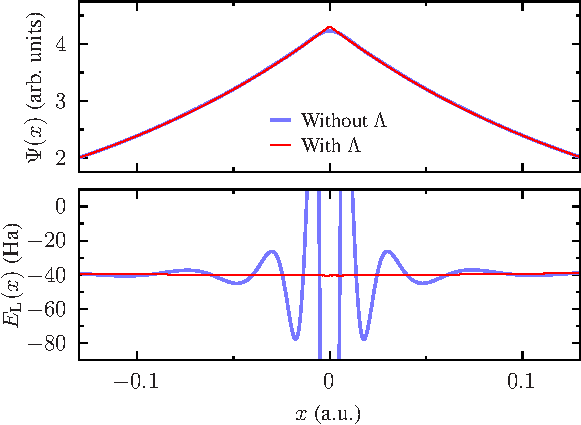
\includegraphics[width=0.8\columnwidth]{figures/optimisation/Fig/cusp-term-eps-converted-to}
    \caption{\gls{HF} wave function value and local energy as a function of the $x$ coordinate of an electron in a carbon atom as it crosses the nucleus at $x=0$, both with and without the $\Lambda$ cusp-correcting Jastrow factor term. This is in the \vdz basis.}
    \label{fig:cusp-term}
\end{figure}

For the calculations in this chapter, we use a total of $44$ optimisable Jastrow factor parameters for the atoms and homonuclear dimers, and $88$ parameters for CN. We keep the $L_v$, $L_\chi$ and $L_f$ cutoff lengths fixed at $4.5$, $4$, and $4$, for simplicity.

\section{Optimisation Strategy}

We optimise $J$ using \gls{VMC}. VMC provides a variational framework in which parameters $\bm \alpha$ present in a trial wave function $\Psi_\mathrm{T}$ can be optimised. In this chapter, $\ket{\Psi_\mathrm{T}} = \e^{J(\bm\alpha)}\ket{D_\mathrm{HF}}$.

Wave function optimisation is usually carried out using a correlated-sampling approach in which a set of $n_mathrm{opt}$ electronic real-space configurations ${\{\bm R}_{i}\}_{i=1}^{n_\mathrm{opt}}$ distributed according to the initial wave function squared, $|\Psi_\mathrm{T}({\bm R}; {\bm \alpha}_0)|^2$ is generated, and then a target function is minimised by varying $\bm\alpha$ at fixed ${\{\bm R}_{i}\}$.

The variational energy estimate for this trial wave function may be written
\begin{equation}
    E_\mathrm{VMC} = \frac{\bra{\Psi_\mathrm{T}} \hat H \ket{\Psi_\mathrm{T}} }{ \braket{\Psi_\mathrm{T}}{\Psi_\mathrm{T}} },
\end{equation}
which may be used as a target function, as presented in section \ref{sec:vmc}.

Another popular target function is the ``variance of the VMC energy,''\todo{citations}
\begin{equation}
\sigma_\mathrm{VMC}^2 = \frac{\bra{\Psi_\mathrm{T}}(\hat H - E_\mathrm{VMC})^2\ket{\Psi_\mathrm{T}}}{\braket{\Psi_\mathrm{T}}},
\end{equation}
which reaches its minimum of zero when the trial wave function is an eigenstate of the Hamiltonian. In practice, minimising $\sigma_\mathrm{VMC}^2$ yields variational energies, but is affected by large fluctuations, as shown in this chapter.

In continuum QMC methods, modifications have been devised to
circumvent this problem, such as weight limiting, unreweighted
variance minimization, or the minimization of other measures of spread
such as the median absolute deviation from the median energy.\supercite{needsVariational2020}

The computational cost of optimizing Jastrow factors within VMC scales
as a small power of system size, typically estimated to be ${\mathcal
O}(N^3)$.

\subsection{Variance of the Reference Energy Minimisation}

In the context of TC, the reference energy
\begin{equation}
    E_\mathrm{ref} = \bra{D_\mathrm{HF}}\e^{-J}\hat H\e^J\ket{D_\mathrm{HF}}
\end{equation}
is of particular significance since it represents the starting point of a TC-FCIQMC calculation (i.e. the walker distributions at imaginary time $\tau=0$ has this energy). It is also the zeroth-order contribution to the TC-\gls{CC} energy.

We refer to its associated variance,
\begin{equation}
  \label{eq:var_eref_1}
  \sigma_\mathrm{ref}^2 =
    \bra{D_\mathrm{HF}}\e^{-J} (\hat H^\dag-E_\mathrm{ref})(\hat H-E_\mathrm{ref}) \e^J\ket{D_\mathrm{HF}}
\end{equation}
as the ``variance of the reference energy,'' which is easily evaluated for a finite VMC sample of size $n_\mathrm{opt}$ as the sample variance of the Slater-Jastrow energy over the HF distribution,
\begin{equation}
    S_\mathrm{ref}^2 =
      \frac 1 {n_\mathrm{opt}-1}
      \sum_{n=1}^{n_\mathrm{opt}}
        \left| \frac {\hat H({\bm R}_n) \Psi_\mathrm{SJ}({\bm R}_n)}
                     {\Psi_\mathrm{SJ}({\bm R}_n)} - {\bar E}_\mathrm{ref}
        \right|^2,
\end{equation}
% TODO : you will want to practice proving this, just in case for your defence
which tends to $\sigma_\mathrm{ref}^2$ as $n_\mathrm{opt}\to\infty$, where $\Psi_\mathrm{SJ}\mathdef \e^JD_\mathrm{HF}$ is the Slater-Jastrow wave function, $\{{\bm R}_n\}_{n=1}^{n_\mathrm{opt}}$ are electronic
configurations distributed according to $D_\mathrm{HF}^2$, and the VMC
estimate of the reference energy is
\begin{equation}
    {\bar E}_\mathrm{ref} =
      \frac 1 {n_\mathrm{opt}}
      \sum_{n=1}^{n_\mathrm{opt}}
        \frac {\hat H({\bm R}_n) \Psi_\mathrm{SJ}({\bm R}_n)}
              {\Psi_\mathrm{SJ}({\bm R}_n)}.
\end{equation}

% TODO: you will want to familiarise yourself with these papers
The variance of the reference energy has been used as a target function for optimising Jastrow factors for the TC method before, albeit in different theoretical frameworks.\todo{citations}

To understand the physical significance of the variance of the reference energy, note that equation \ref{eq:var_eref_1} may be rewritten as
\begin{equation}
    \label{eq:varref-connectivity}
    \sigma_\mathrm{ref}^2 = \sum_{I\neq \mathrm{HF}}\bra{D_I}\htc\ket{D_\mathrm{HF}},
\end{equation}
where $I$ runs over a complete basis set.\footnote{Here we have a complete basis set because we are optimising with continuum Monte Carlo. If we were to optimise this by directly calculating the matrix elements in equation \ref{eq:varref-connectivity}, then the sum must be truncated. This is the subject of ongoing work.}

As evident by equation \ref{eq:varref-connectivity}, minimising $\sigma_\mathrm{ref}^2$ essentially amounts to minimising the coupling of the reference determinant with the remainder of the space, which in the context of FCIQMC translates to a reduced spawning rate from the reference determinant to its connected excited-state determinants, thereby increasing the amplitude of the reference determinant in the resulting CI vector.

Note also that if the Slater-Jastrow wave function were an exact eigenstate of $\hat H$, then a TC-FCIQMC simulation starting from the HF determinant would immediately converge to a strictly single-determinant solution. Although this ideal scenario cannot be achieved in practice, it nevertheless illustrates the potential benefits of obtaining a relatively single-reference CI solution by minimising this target function. We expect that this increased single-reference character will also benefit other approaches, particularly those based on single references, such as TC-CC.

We therefore investigate the performance of minimising the variance of the reference as an alternative to minimising the variance of the VMC energy. In figure \ref{fig:varmin-E-Eref}, we compare the VMC energy and variance obtained by variance minimisation methods along with energy-minimised \todo{citations} results for reference, for the systems considerd in this chapter, using $n_\mathrm{opt}=10^5$ VMC configurations.

\begin{figure}[htbp]
    \centering
    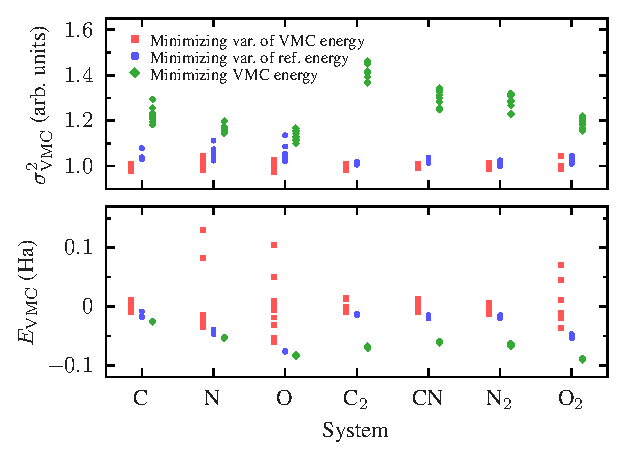
\includegraphics[width=0.8\textwidth]{figures/optimisation/Fig/varmin-E-Eref}
    \caption{Variance of the VMC energy (top) and VMC energy (bottom) of the systems considered in this chapter using the \vtz basis and Jastrow factors obtained by minimising the variance of the VMC energy (red squares), the variance of the reference energy (blue circles), or the VMC energy (green diamonds) in each of ten independent optimisation runs with $n_\mathrm{opt}=10^5$ VMC configurations. To ease comparisons, variances have been rescaled and energies shifted by their average values from minimising the variance of the VMC energy (i.e. the red squares average to a variance of $1$ and an energy of $0$ in the plot). The subpar ability of VMC energy variance minimisation to yield consistent VMC energies is evident in the bottom panel, suggesting to use the variance of the reference.}
    \label{fig:varmin-E-Eref}
\end{figure}
%
Minimizing the variance of the VMC energy produces lower average
values of $\sigma_\mathrm{VMC}^2$, as one would expect, but also erratic
VMC energies with very large standard deviations (up to $\sim50$ mHa
in our tests).
%
Minimizing the variance of the reference energy, on the other hand,
produces values of $\sigma_\mathrm{VMC}^2$ which are only slightly higher
on average than those obtained from minimizing the variance of the VMC
energy ($1$--$5\%$ in our tests), while producing more stable VMC
energies with much smaller standard deviations (up to $\sim3$ mHa in
our tests).
%
We therefore do not use ``regular'' variance minimization since it
introduces large stochastic noise, making it unsuitable for optimizing
Jastrow factors, and from this point on we use the term ``variance
minimization'' to refer to the minimization of the variance of the
reference energy.

\subsection{Choosing an Appropriate Sample Size}

While expectation values relevant for most continuum QMC calculations converge using relatively few VMC configurations, it has also been known\todo{citation Spink} that in order to converge other quantities, far more configurations are needed. That is, $n_\mathrm{opt}$ is larger. In the spirit of \gls{MC}, we may estimate the convergence of the expectation value for some quantity by performing multiple optimisation runs with different random number seeds but otherwise the same inputs. This would give us a standard deviation.

The value we want to converge in this case is not the VMC energy, nor the reference energy, but instead the TC-FCI energy. In practice, we use the uncertainty of the VMC estimate of the reference energy $\bar E_\mathrm{ref}$ as a proxy for the standard deviation of the TC-FCIQMC energy. This is justified because:
\begin{itemize}
    \item The standard deviation of the TC-FCIQMC energy is not larger than the standard deviation of the reference energy, as illustrated in figure \ref{fig:spread_c2_cc-pvdz}. It is usually significantly smaller thanks to the ability of TC-FCIQMC to conpensate for the presence of a bias in $E_\mathrm{ref}$ via the correlation energy.
    \item The standard deviation of the reference energy is not larger than the statistical uncertainty of the VMC estimate of the reference energy obtained with $n_\mathrm{opt}$ configurations. It is usually significantly smaller due to the use of variance reduction techniques in QMC.
\end{itemize}

\begin{figure}[htbp]
    \centering
    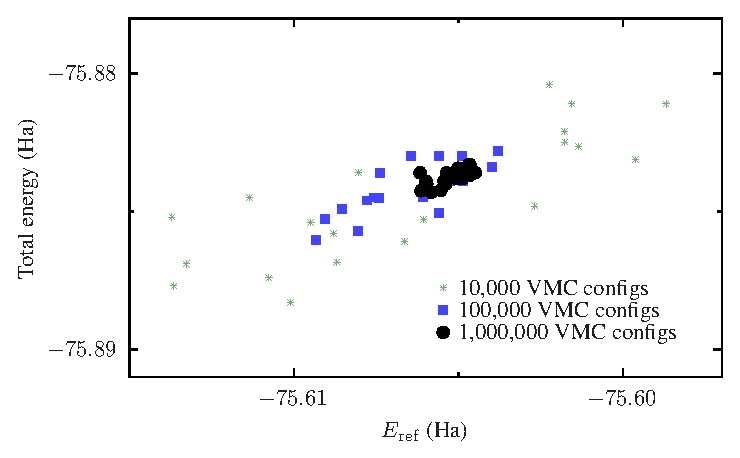
\includegraphics[width=0.8\textwidth]{figures/optimisation/Fig/spread_c2_cc-pvdz}
    \caption{TC-FCIQMC energy of the C$_2$ molecule using $10^6$ walkers with the \vdz basis as a function of the reference energy for multiple independent Jastrow factor parameter sets obtained by variance minimisation using three different VMC sample sizes. The horizonal spread is about $1.8$ times larger than the vertical spread, in line with the expectation that the standard deviation of the TC-FCIQMC energy is smaller than that of the reference energy.}
    \label{fig:spread_c2_cc-pvdz}
\end{figure}

For the atoms and molecules considered in this chapter, we use $n_\mathrm{opt}=2\times 10^7$ to yield TC-FCIQMC energies with standard deviations of less than $0.1$ mHa.

\subsection{Energy Minimisation}

The obvious alternative to variance minimisation is minimising the VMC energy,\todo{citations} which, as already demonstrated in figure \ref{fig:varmin-E-Eref}, results in lower VMC energies but higher VMC variances.
Energy minimisation yields wave functions which minimise the statistical fluctuations of the local energy in DMC calculations\todo{citation} and is the typical choice for continuum QMC. However, for our purposes, it is unclear whether the resulting wave functions provide a better description of the system than those produced by variance minimisation.

In figure \ref{fig:bsdep-atoms-emin}, we compare the convergence with basis-set size of TC-FCIQMC total energies of the C, N, and O atoms using energy- and variance-minimised Jastrow factors. Variance minimisation appears to produce wave functions which converge quickly and largely variationally to the basis set limit, which energy-minimised wave functions tend to yield non-variational TC-FCIQMC energies which converge more slowly to the basis set limit.

\begin{figure}[htbp]
    \centering
    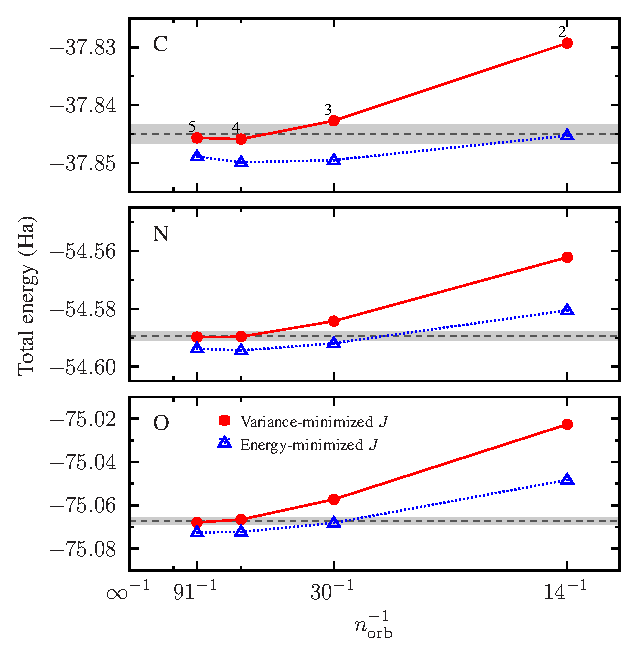
\includegraphics[width=0.8\textwidth]{figures/optimisation/Fig/bsdep-atoms-emin}
    \caption{Total energy of the C, N, and O atoms as a function of the reciprocal number of molecular orbitals in the \vxz{X} basis set family. The non-variational behaviour of up to about $5$ mHa is evident for the energy-minimised Jastrow factors, for which convergence to the exact energy as a function of basis-set size is slow. The shaded areas represent $\pm 1$ kcal/mol (so-call ``chemical accuracy'') around the exact non-relativistic total energy from reference \todo{citation}. Points in the top panel are annotated with the basis set cardinal number $X$.}
    \label{fig:bsdep-atoms-emin}
\end{figure}

In figure \ref{fig:bsdep-dimers-emin} we plot the atomisation energies of the dimers as a function of reciprocal basis-set size, again demonstrating variance-minimised Jastrow factors exhibit favourable convergence properties.

\begin{figure}[htbp]
    \centering
    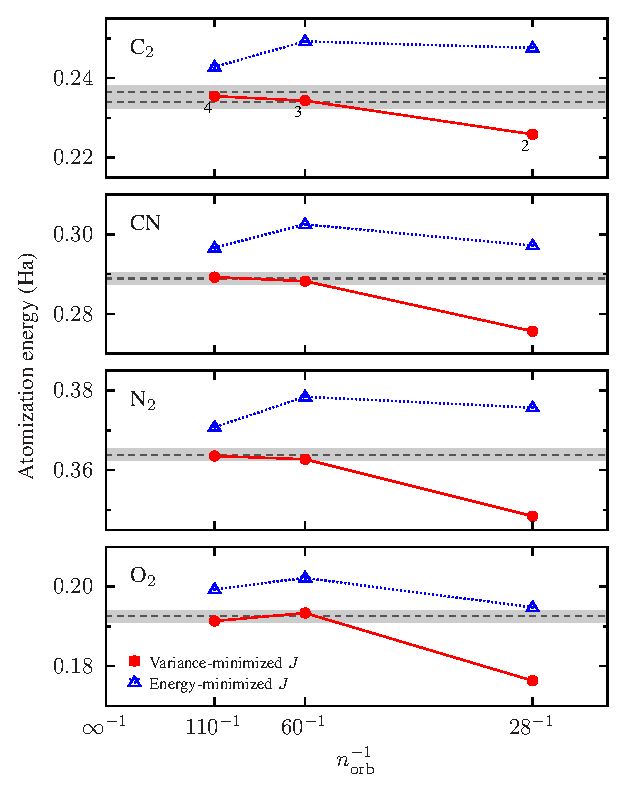
\includegraphics[width=0.8\textwidth]{figures/optimisation/Fig/bsdep-dimers-emin}
    \caption{Atomisation energy of the C$_2$, CN, N$_2$, and O$_2$ molecules as a function of the reciprocal of the number of molecular orbitals using the \vxz{X} family of basis sets and Jastrow factors obtained by variance and energy minimisation. The shaded areas represent $\pm 1$ kcal/mol around the theoretical estimate of the exact non-relativistic atomisation energies from references \todo{citations}}.
    \label{fig:bsdep-dimers-emin}
\end{figure}

Considering this evidence, we choose to use variance minimisation to optimise the Jastrow factors for subsequent post-HF calculations.

\section{Grid Sizes}

How matrix elements are evaluated is presented in appendix \ref{chap:pytchint}. As mentioned there, we use Treutler-Ahlrichs integration grids,
\todo{citations} which are atom-centred
grids constructed as the combination of a radial grid running up to
the Bragg radius and a Lebedev angular grid. These are obtained using \pyscf, which provides an integer parameter $l_\mathrm{grid}$ to control the grid density. Here we test grid errors by evaluating TC-FCIQMC energies at $l_\mathrm{grid}=1$--$5$ and defining the integration error as the difference of each of these results with the value obtained by linear extrapolation to the $1/n_\mathrm{grid}\to 0$ limit.

In figure \ref{fig:griderr-atoms} we plot the absolute integration error in the total energy of the atoms as a function of $1/n_\mathrm{grid}$ for \vdz, \vtz and \vqz basis sets. We find that the basis set size has little to no effect on the integration error.

\begin{figure}[htbp]
    \centering
    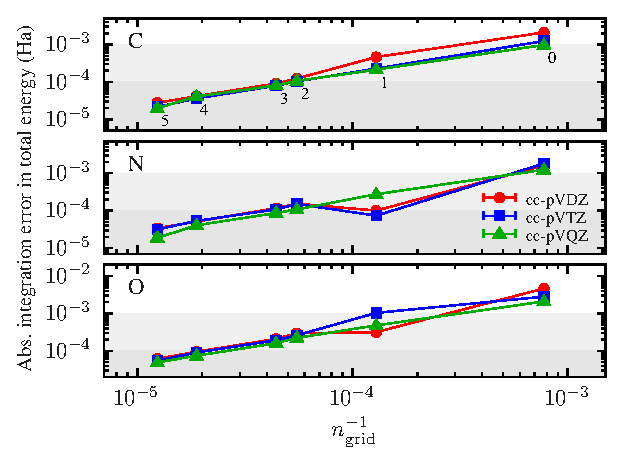
\includegraphics[width=0.8\textwidth]{figures/optimisation/Fig/griderr-atoms}
    \caption{Absolute integration errors in the total energy for the C, N, and O atoms as a function of the reciprocal of grid size using basis sets in the \vxz{X} family. The gray areas correspond to integration errors of less than $1$ and $0.1$ mHa. Points in the top panel are annotated with the value of \pyscf's grid density parameter.}
    \label{fig:griderr-atoms}
\end{figure}

In figure \ref{fig:griderr-dimers} we plot the absolute integration error in the total energies of the molecules, the atoms that conform them, and atomisation energies using the \vdz basis. We find integration-error cancellation in energy differences, with atomisation energy for all four molecules reaching $0.1$ mHa for $l_\mathrm{grid}=2$. This represents a $60$-point radial grid combined with a $302$-point angular grid, for a total of $18120$ grid points per atom. We use this throughout this dissertation.

\begin{figure}[htbp]
    \centering
    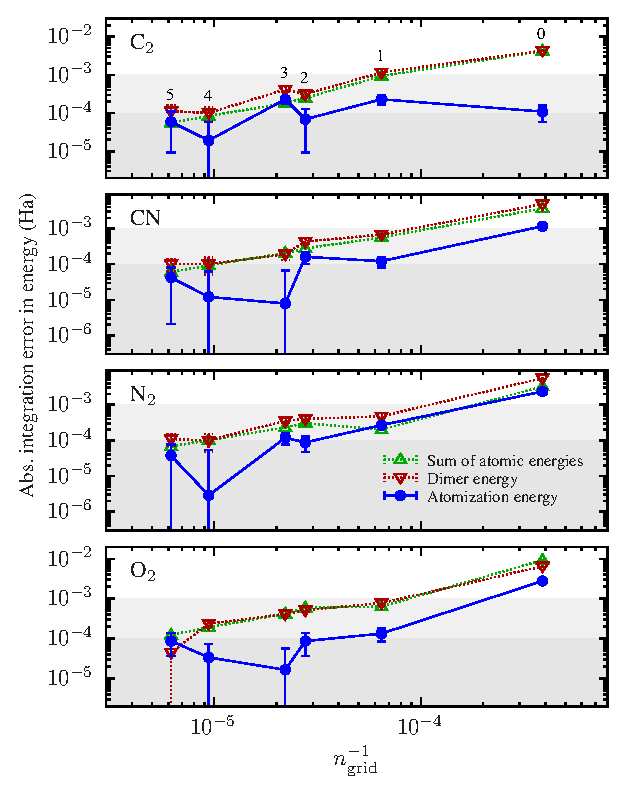
\includegraphics[width=0.8\textwidth]{figures/optimisation/Fig/griderr-dimers}
    \caption{Absolute integration error in the energy as a function of the reciprocal number of grid points used for the evaluation of TC integrals. The shaded areas correspond to integration errors of less than $1$ and $0.1$ mHa. Points in the top panel are annotated with the value of \pyscf's grid density parameter. These results demonstrate that $l_\mathrm{grid}=2$ is sufficient to achieve sub-mHa accuracy in total energies and sub-$0.1$-mHa accuracy in relative energies.}
    \label{fig:griderr-dimers}
\end{figure}


\section{Compactification of the CI Vector}
The more compact the CI wave function is, the easier it is for FCIQMC to sample the wave function accurately and the smaller the initiator error becomes. The TC method has already been shown to make CI wave functions more compact for the two-dimensional Hubbard model.\todo{citation} Let $\{c_I\}$ be the $L^2$-normalized coefficients of the CI wave
function such that $\sum_I c_I^2=1$.
%
The quantity
%
\begin{equation}
  \label{eq:xi_compactness}
  \xi = \frac { c^\mathrm{(TC)}_\mathrm{HF} - c^\mathrm{(non-TC)}_\mathrm{HF} }{ 1 - c^\mathrm{(non-TC)}_\mathrm{HF} }
\end{equation}
%
is then a measure of the enhancement in the compactness of the wave
function, going from $0$ for no enhancement to $1$ if the TC wave
function becomes exactly single-determinantal.

From reference \todo{citation}, TC yields a maximum of $\xi=0.64$ for the 18-site 2D Hubbard model. We find that the values of $\xi$ for atomic and molecular systems are not dissimilar from this, as shown in table \ref{table:l2_norms}.
%
\begin{table}[htbp]
    \centering
    \begin{tabular}{cccccccc}
            & C      & N      & O      &
              C$_2$  & CN     & N$_2$  & O$_2$  \\
    \hline \hline
    cc-pVDZ & $0.46$ & $0.63$ & $0.71$
            & $0.14$ & $0.23$ & $0.38$ & $0.53$ \\
    cc-pVTZ & $0.45$ & $0.61$ & $0.69$
            & $0.15$ & $0.24$ & $0.40$ & $0.55$ \\
    cc-pVQZ & $0.44$ & $0.60$ & $0.69$
            & $0.15$ & $0.24$ & $0.41$ & $0.57$ \\
    \hline
    \end{tabular}
    \caption{
      Enhancement of the compactness of the CI wave function, $\xi$ in
      Eq.\ \ref{eq:xi_compactness}, between our non-TC and TC-FCIQMC
      calculations.
    }
    \label{table:l2_norms}
  \end{table}

\section{Neglecting Three-Body Excitations}

As described in section \ref{sec:fciqmc}, sampling in FCIQMC involves spawning walkers from occupied determinants onto connected determinants. The $\hat L$ matrix, that is the three-body operator arising from the similarity transformation in TC, results in TC also connecting determinants by three-body excitations. This represents a huge increase in the connectivity of the Hilbert space compared to non-TC-FCIQMC.

These three-body excitations are represented by $L_{ijk}^{abc}$ where each index is distinct. These have been found to typically be small\todo{citation}. Moreoever, simultaneous interaction of three electrons is unlikely due to Pauli repulsion (as necessarily at least two of the electrons will be of the same spin). Therefore, we neglect these contributions. The only distinct six-index integrals that we must keep are those occupied in the HF determinant, as these matrix elements are necessary to evaluate the projected energy.

Neglecting pure three-body excitations reduces the amount of storage needed to hold $\hat L$ from $\mathcal{O}(M^6)$ to $\mathcal{O}(M^5+N^3M^3)$, where $M$ is the number of orbitals and $N$ is the number of electrons. Reduction factors obtains for the molecules studied in this chapter are reported in table \ref{table:no3_memory}.

\begin{table}[htbp]
    \centering
    \begin{tabular}{cccccccc}
            & C      & N      & O      &
              C$_2$  & CN     & N$_2$  & O$_2$  \\
    \hline \hline
    cc-pVDZ & $1.23$ & $1.17$ & $1.17$ &
              $1.87$ & $1.78$ & $1.78$ & $1.58$ \\
    cc-pVTZ & $2.04$ & $2.02$ & $1.93$ &
              $3.72$ & $3.66$ & $3.66$ & $3.46$ \\
    cc-pVQZ & $3.31$ & $3.44$ & $3.13$ &
              $6.60$ & $6.54$ & $6.57$ & $6.41$ \\
    \hline
    \end{tabular}
    \caption{
      $\hat L$ matrix storage reduction factor from neglecting
      pure three-body excitations, computed as the number of
      non-zero matrix elements in a the full $\hat L$ matrix
      divided by the number of non-zero matrix elements with
      repeated indices or three or more indices corresponding to
      orbitals occupied in the HF determinant.
    }
    \label{table:no3_memory}
\end{table}

Since two-body excitations are typically more expensive to attempt in practice compared to triple excitations, neglecting the latter actually increases the cost per step of the calculation. However, neglecting pure three-body excitations allows the TC-FCIQMC time step to be larger, thereby resulting in reduced serial correlation in the statistics, which enables reaching the target accuracy in fewer time steps, so one can expect a net cost reduction thanks to this approximation. Walltime reduction factors for the molecules studied in this chapter are reported in table \ref{table:no3_cost}.
\begin{table}[htbp]
    \centering
    \begin{tabular}{cccccccc}
            & C     & N     & O     &
              C$_2$ & CN    & N$_2$ & O$_2$ \\
    \hline \hline
    cc-pVDZ & $0.9$ & $1.0$ & $1.1$ &
              $1.7$ & $1.2$ & $1.5$ & $1.6$ \\
    cc-pVTZ & $1.0$ & $1.0$ & $0.8$ &
              $2.4$ & $1.0$ & $1.8$ & $2.0$ \\
    cc-pVQZ & $1.5$ & $1.5$ & $1.0$ &
              $3.1$ & $0.9$ & $1.9$ & $2.3$ \\
    \hline
    \end{tabular}
    \caption{
      Reduction factor in the walltime required to advance one unit of
      imaginary time at fixed population from neglecting pure three-body
      excitations in the TC-FCIQMC calculation.
      %
      \label{table:no3_cost}}
\end{table}

The effect of neglecting these pure three-body excitations on atomisation energy is also small, as shown in table \ref{table:no3_Eat_error}. We find that this approximation results in errors of the order of
$\sim0.3$ mHa at the cc-pVTZ level, which is a relatively small bias
considering the substantial storage and cost benefits of the
approximation.

\begin{table}[htbp]
    \centering
    \begin{tabular}{cllll}
                              &
    \multicolumn{1}{c}{C$_2$} &
    \multicolumn{1}{c}{CN   } &
    \multicolumn{1}{c}{N$_2$} &
    \multicolumn{1}{c}{O$_2$} \\
    \hline \hline
    cc-pVDZ   & $-0.62(2)$ & $-0.46(0)$ & $-0.56(2)$ & $-0.55(2)$ \\
    cc-pVTZ   & $-0.36(5)$ & $-0.30(2)$ & $-0.32(5)$ & $-0.20(3)$ \\
    cc-pVQZ   & $-0.45(6)$ & $-0.21(2)$ & $-0.32(7)$ & $-0.27(5)$ \\
    \hline
    \end{tabular}
    \caption{
      Error in the atomization energy of the molecules considered in this
      work incurred by neglecting pure three-body excitations from the
      FCIQMC dynamics, in mHa.
      %
      \label{table:no3_Eat_error}}
  \end{table}

\section{Atomisation Energies}

In this section, we compare results of TC-FCIQMC with individually variance-optimised Jastrow factors as a function of basis-set size with the corresponding non-TC results and with benchmark \gls{CBS} values from references \todo{citations}.

Table \ref{table:total_energies} shows a list of total energies obtained for each system and basis set.
\begin{table*}[htbp!]
    \centering
    \begin{tabular}{c|cccc}
      \multicolumn{2}{c}{~} &
      \multicolumn{1}{c}{C} &
      \multicolumn{1}{c}{N} &
      \multicolumn{1}{c}{O} \\
      \hline \hline
      \multicolumn{4}{c}{~} \\[-0.4cm]
      \parbox[t]{2mm}{\multirow{5}{*}{\rotatebox[origin=c]{90}{non-TC}}}
      &cc-pVDZ& $ -37.7619$ & $ -54.4801$ & $ -74.9117$ \\
      &cc-pVTZ& $ -37.7900$ & $ -54.5252$ & $ -74.9853$ \\
      &cc-pVQZ& $ -37.8126$ & $ -54.5535$ & $ -75.0236$ \\
      &cc-pV5Z& $ -37.8199$ & $ -54.5627$ & $ -75.0369$ \\
      &cc-pV6Z& $ -37.8263$ & $ -54.5697$ & $ -75.0447$ \\
      \multicolumn{4}{c}{~} \\[-0.3cm]
      \parbox[t]{2mm}{\multirow{4}{*}{\rotatebox[origin=c]{90}{TC}}}
      &cc-pVDZ& $ -37.8293$ & $ -54.5622$ & $ -75.0226$ \\
      &cc-pVTZ& $ -37.8427$ & $ -54.5842$ & $ -75.0572$ \\
      &cc-pVQZ& $ -37.8459$ & $ -54.5896$ & $ -75.0665$ \\
      &cc-pV5Z& $ -37.8457$ & $ -54.5898$ & $ -75.0678$ \\
      \multicolumn{4}{c}{~} \\[-0.3cm]
      \multicolumn{2}{c}{Ref.\ byta!!} % \todo{citationBytautas2005}
              & $ -37.8450$ & $ -54.5893$ & $ -75.0674$ \\
      \multicolumn{2}{c}{Ref.\ hard!!} % \todo{citationHardingHEAT2008}
              & $ -37.8450$ & $ -54.5893$ & $ -75.0674$ \\
      \hline
    \end{tabular}

    \vspace{1em}

    \begin{tabular}{c|ccccc}
      \multicolumn{2}{c}{~} &
      \multicolumn{1}{c}{C$_2$} &
      \multicolumn{1}{c}{CN} &
      \multicolumn{1}{c}{N$_2$} &
      \multicolumn{1}{c}{O$_2$} \\
      \hline \hline
      \multicolumn{5}{c}{~} \\[-0.4cm]
      \parbox[t]{2mm}{\multirow{4}{*}{\rotatebox[origin=c]{90}{non-TC}}}
      &cc-pVDZ& $ -75.7320$ & $ -92.4970$ & $-109.2809$ & $-149.9915$ \\
      &cc-pVTZ& $ -75.8094$ & $ -92.5954$ & $-109.4014$ & $-150.1554$ \\
      &cc-pVQZ& $ -75.8578$ & $ -92.6517$ & $-109.4653$ & $-150.2362$ \\
      &cc-pV5Z& $ -75.8752$ & $ -92.6717$ & $-109.4881$ & $-150.2655$ \\
      \multicolumn{5}{c}{~} \\[-0.3cm]
      \parbox[t]{2mm}{\multirow{4}{*}{\rotatebox[origin=c]{90}{TC}}}
      &cc-pVDZ& $ -75.8844$ & $ -92.6671$ & $-109.4727$ & $-150.2216$ \\
      &cc-pVTZ& $ -75.9197$ & $ -92.7152$ & $-109.5312$ & $-150.3078$ \\
      &cc-pVQZ& $ -75.9272$ & $ -92.7247$ & $-109.5428$ & $-150.3244$ \\
      \multicolumn{5}{c}{~} \\[-0.3cm]
      \multicolumn{2}{c}{Ref.\ fell!!} % \todo{citationFeller2008}
              & $ -75.9240$ & $ -92.7232$ & $-109.5425$ & $-150.3273$ \\
    \multicolumn{2}{c}{Ref.\ byta!!} % \todo{citationBytautas2005}
      & $ -75.9265$ &             & $-109.5427$ & $-150.3274$ \\
      \multicolumn{2}{c}{Ref.\ hard!!} % \todo{citationHardingHEAT2008}
      &             & $ -92.7229$ & $-109.5425$ & $-150.3275$ \\
      \hline
    \end{tabular}

    \caption{Total energies in Ha obtained for atoms (top) and molecules (bottom) considered in this work, along with benchmark non-relativistic results. Statistical uncertainties from Monte Carlo sampling are smaller than $0.0001$ Ha.}
    \label{table:total_energies}
\end{table*}
%
We find the TC total energies to be remarkably accurate already at the
cc-pVQZ basis set level, differing by less than $2$ mHa per atom from
benchmark CBS values, while the non-TC total energies still miss the
benchmarks by $25$--$30$ mHa per atom with the cc-pV5Z basis set, and
$20$ mHa per atom at the cc-pV6Z level. The TC total energies exhibit slightly non-variational convergence, with the atomic energies reaching values $0.5$ mHa below the benchmark before increasing again towards it for larger basis-set sizes. While non-variationality is undesirable in a method, the amount by which the TC results dip below the \gls{CBS} limit is sufficiently small for this not to be an issue in practice.

From a chemical perspective, relative energies are more important than totaly energies. The atomisation energies of the C$_2$, CN, N$_2$, and O$_2$ molecules
obtained from the total energies in table \ref{table:total_energies}
are given in table \ref{table:atomization}
and plotted in figure
\ref{fig:bsdep-dimers-nontc}.
%
\begin{table}[htbp!]
  \centering
  \begin{tabular}{c@{\;\;}|@{\;\;}crrrr}
    \multicolumn{2}{c}{}      &
    \multicolumn{1}{c}{C$_2$} &
    \multicolumn{1}{c}{CN}    &
    \multicolumn{1}{c}{N$_2$} &
    \multicolumn{1}{c}{O$_2$} \\
    \hline \hline
    \multicolumn{6}{c}{} \\[-0.4cm]
    \parbox[t]{2mm}{\multirow{4}{*}{\rotatebox[origin=c]{90}{non-TC}}}
    &cc-pVDZ& $208.2$ & $255.0$ & $320.7$ & $168.0$ \\
    &cc-pVTZ& $229.4$ & $280.1$ & $351.0$ & $184.9$ \\
    &cc-pVQZ& $232.6$ & $285.6$ & $358.4$ & $189.0$ \\
    &cc-pV5Z& $235.5$ & $289.2$ & $362.6$ & $191.7$ \\
    \multicolumn{6}{c}{} \\[-0.3cm]
    \parbox[t]{2mm}{\multirow{3}{*}{\rotatebox[origin=c]{90}{TC}}}
    &cc-pVDZ& $225.9$ & $275.6$ & $348.4$ & $176.4$ \\
    &cc-pVTZ& $234.3$ & $288.2$ & $362.7$ & $193.4$ \\
    &cc-pVQZ& $235.5$ & $289.3$ & $363.6$ & $191.4$ \\
    \multicolumn{6}{c}{} \\[-0.3cm]
    \multicolumn{2}{c}{Ref.\ \todo{...}} % \onlinecite{Feller_molecules_2008}
            & $234.0$ & $288.9$ & $363.9$ & $192.5$ \\
    \multicolumn{2}{c}{Ref.\ \todo{...}} % onlinecite{Bytautas_diatomic_2005}
            & $236.5$ &         & $364.1$ & $192.6$ \\
    \multicolumn{2}{c}{Ref.\ \todo{...}} % \onlinecite{Harding_HEAT_2008}
            &         & $288.6$ & $363.9$ & $192.7$ \\
    \hline
  \end{tabular}
  \caption{Atomisation energies in mHa obtained for the molecules
    considered in this chapter, along with benchmark non-relativistic
    results.
    %
    Statistical uncertainties arising from Monte Carlo sampling
    are smaller than $0.1$ mHa in all cases.
  }
  \label{table:atomization}
\end{table}
%
\begin{figure}[!hbt]
  \begin{center}
    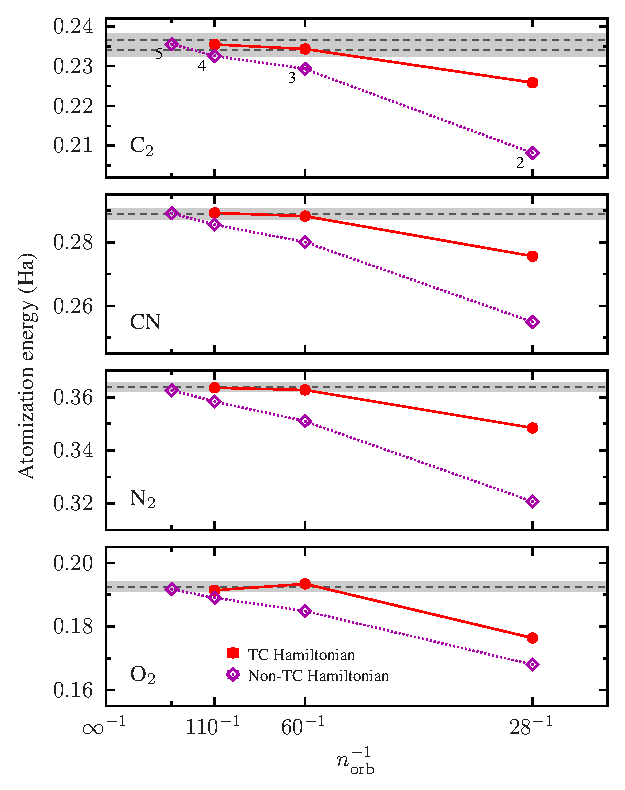
\includegraphics[width=0.8\textwidth]{figures/optimisation/Fig/bsdep-dimers-nontc}
    \caption{
      Atomisation energy of the C$_2$, CN, N$_2$, and O$_2$ molecules
      obtained with FCIQMC and TC-FCIQMC as a function of the
      reciprocal of the number of molecular orbitals using the
      \vxz{X} family of basis sets.
      %
      Points in the top panel are annotated with the basis set
      cardinal number $X$.
      %
      The shaded areas represent $\pm 1$ kcal/mol around the
      theoretical estimate of the non-relativistic atomisation energy
      of \todo{Feller citation}; the distinct
      estimate of \todo{Bytautas citation} is also
      shown for C$_2$.
    }
    \label{fig:bsdep-dimers-nontc}
  \end{center}
\end{figure}

As with the total energies, we find that the TC atomisation energies converge much faster with respect to basis-set size compared to the non-TC calculations. In fact, the TC results are already chemically accurate at the \vtz basis-set level, matching accuracy of \vxz{5} non-TC results. The application of the TC method to quantum chemical methods in
general could be presumed to be problematic because any theoretical
guarantee of cancellation of errors in energy differences disappears
with the introduction of separately-optimized Jastrow factors for each
system.
%
However, the fact that in our results the relative energy converges at
smaller basis-set sizes than the total energy implies that substantial
error cancellation is at play in practice.

\section{Conclusion and Outlook}

In this chapter, we presented a new method to optimise flexible Jastrow factors of a form common in continuum QMC methods for applications to TC. We tested these within the TC-FCIQMC framework. Minimising the variance of the reference energy is shown to be especially good for the TC method, since it maximises the single-reference character of the CI wave function.

These results show that this workflow can provide remarkably accurate total and relative energies, with relative energies at \vtz rivalling non-TC results at \vxz{5}. These results also provide better energy estimates compared to other promising methods, such as neural-network based trial wave functions.\todo{citations}

Future work on this topic have focused on technical advancements and efficient approximations for dealing with the three-body integrals.

\subsection{The xTC Approximation}

One particularly significant refinement of this method is the so-called ``xTC approximation,''\supercite{christlmaierXTC2023} wherein upon neglecting explicit three-body contributions, the remaining three-body terms are ``folded'' into the remaining lower-order terms.

The Hamiltonian is normal-ordered with respect to $\Phi$ (where $\Psi=\e^J\Phi$, $\Phi$ being the HF determinant in this chapter)\todo{citations}

\begin{equation}
    H_N = \htc - \bra{\Phi}\HTC\ket\Phi = F_N + V_N + L_N
\end{equation}
where the one-, two-, and three-body operators are (using Einstein summation)\todo{check these equations}
\begin{align}
F_N =& [h_q^p + (U_{qs}^{pr}-U_{sq}^{pr})\gamma_s^r \\
&- \frac 12 (L_{qsu}^{prt} - L_{qus}^{prt}-L_{usq}^{prt})\gamma_{us}^{rt}]
\tilde a_q^p, \\
V_N =& \frac 12[U_{qs}^{pr} - (L_{qsu}^{prt} - L_{qus}^{prt}-L_{usq}^{prt})]\tilde a_{qs}^{pr}, \\
L_N =& \frac 16L_{qsu}^{prt}\tilde a_{qsu}^{prt}
\end{align}
and $U=V-K$, $\tilde a_{p\dots}^{q\dots}$ are the normal ordered
excitation operators, and $\gamma_{p\dots}^{q\dots}=\bra\Phi a_{p\dots}^{q\dots}\ket\Phi$ are the density matrices.

Ignoring the three-body terms $L_N$ leads to an improved scaling with respect to basis set size while directly contracting intermediates to the lower-body corrections obviates the necessity to calculate $L$ and results in excellent energy agreement.\supercite{christlmaierXTC2023} Once the integrals are calculated, $\htc$ has, like $\hat H$, at most two-body interactions and therefore needs storage for four indices (albeit we no longer have Hermiticity). This means that calculations done on these integrals (in principle) are not much more expensive than the conventional non-TC calculations.

\label{sec:xtc}
